\documentclass[12pt,titlepage]{article}

\usepackage[utf8]{inputenc}
\usepackage[ngerman]{babel}
\usepackage{cite}
\usepackage[a4paper,lmargin={2.5cm},rmargin={2.5cm},
tmargin={2.5cm},bmargin = {4cm}]{geometry}
\usepackage{amsmath}
\usepackage{enumitem}
\usepackage{graphicx}
\usepackage{listings}
\usepackage{color}
\usepackage{caption,tabularx,booktabs}
\usepackage{multirow}
\usepackage{here}
\usepackage{float}
\usepackage{fancyhdr}
\usepackage{lmodern}
\usepackage{blindtext}
\usepackage{mathtools}
\usepackage{amsmath}

\begin{titlepage}
\author{Knoll Alexander }
\title{Iterative Verfahren}
\date{\today}
\end{titlepage}

\pagestyle{fancy}
%
\makeatletter
\let\runauthor\@author
\lhead{Numerik 2}
\chead{}
\rhead{
\includegraphics[height=50px]{hmlogo}}
\setlength\headheight{40px}
\setlength{\parindent}{0pt} % Neue Absätze werden nicht eingerückt

%
\lfoot{}
\cfoot{\thepage}
\rfoot{\runauthor}
\makeatother
%%%%%%%%%%%%%%%%%%%%%%%%%%%%%%%%%%%%%%%%%%%%%%%%%
%     Neue Befehle werden hier definiert        %
%%%%%%%%%%%%%%%%%%%%%%%%%%%%%%%%%%%%%%%%%%%%%%%%%

\renewcommand{\headrulewidth}{0.4pt}
\renewcommand{\footrulewidth}{0.4pt}
\newcommand{\norm}[1]{\lvert #1 \rvert}


\lstloadlanguages{Python}
\lstset{numbers=left,stepnumber=1,frame=single,language=Python,
        basicstyle=\scriptsize\ttfamily,numberstyle=\scriptsize,
        commentstyle=\upshape\ttfamily,
        numbersep=7pt,tabsize=2,breaklines=false,
        morecomment=[l]{//},showtabs=false,showspaces=false,
        showstringspaces=false,extendedchars=true,inputencoding={utf8},
        keywordstyle=\bfseries\color{darkblue},stringstyle=\color{darkred}}
\newcommand{\pp}[1]{\phantom{#1}}

% diese zeile ermöglicht aufzählungen über buchstaben
% \renewcommand{\theenumi}{\Alph{enumi}}

\newcommand\Section[1]{ %
  \addtocontents{toc}{\protect\setcounter{tocdepth}{0}}
  \subsubsection*{#1}
  \addtocontents{toc}{\protect\setcounter{tocdepth}{3}}}
\definecolor{darkblue}{rgb}{0,0,.6}
\definecolor{darkred}{rgb}{.6,0,0}
\definecolor{darkgreen}{rgb}{0,.6,0}
\definecolor{red}{rgb}{.98,0,0}
\renewcommand{\refname}{Literaturverzeichnis}
\renewcommand{\contentsname}{Inhaltsverzeichnis}

\begin{document}

\maketitle

\part*{Euler-Bernoulli-Balken}

	Der Euler-Bernoulli-Balken ist ein einfaches Modell für eine Biegevorgang auf Grund von
	Spannung. Bezeichnet $y(x)$ für $0 \leq x \leq L$ die vertikale Auslenkung, so gilt
	$EIy (x) = f (x)$ wobei $E$ eine Material-Konstante und $I$ das Trägheitsmoment ist. 
	$f(x)$ beschreibt als Kraft pro Einheitslänge die Beladung des Balkens. Durch Diskretisierung erhält man aus der Differentialgleichung ein lineares Gleichungsystem, das hier iterativ gelöst werden soll.
	
	Betrachtet wird dabei ein Stahlträger der Länge $L = 10m$ mit Tiefe $d = 5cm$ und Breite $b = 10cm$. Die Dichte von Stahl ist ungefähr $7850 \frac{kg}{m^3}$, 
	$E = 2 \cdot 10^11 \frac{N}{m^2}$, $I = \frac{bd^3}{12}$

\section{Unbelasteter Balken}

	Zunächst soll ein an beiden Seiten aufliegender Balken untersucht werden.
	Somit gilt $y(0) = y'(x0) = y(L) = y'(L) = 0 $.\newline
	Um entscheiden zu können welches Verfahren zur Lösung des Problems geeignet ist, müssen diese auf Konvergenz untersucht werden. Das Problem ist gegeben durch
	\begin{equation}
		Ax = \frac{h^4}{EI}f,
	\end{equation}
	
	wobei $h = \frac{L}{n+1}$ und $f = g \cdot f(x)$ gilt. Um zu prüfen ob eines der Verfahren konvergiert muss $A$ gewisse eigenschaften besitzen. Die Verfahren konvergieren, wenn eine der folgenden Bedingungen erfüllt ist.
	
	\begin{itemize}
		\centering
		\item Jacobi Verfahren
		\begin{itemize}
			\centering	
			\item Diagonaldominanz
		\end{itemize}
		\item Gauß-Seidel Verfahren
		\begin{itemize}
			\centering
			\item Diagonaldominanz
			\item Positiv-definit
		\end{itemize}
	\end{itemize}
	
	\subsection{Konvergenzuntersuchung}
		
		\subsubsection{Diagonaldominanz}
			Beide Verfahren konvergieren sobald $A$ diagonaldominant ist. Speziel
			für die gegebene Matrix lässt sich sagen, dass dies nicht der Fall ist.
			Für strikte Diagonaldominanz muss gelten
			\begin{equation*}
				\sum_{j = 1, j \neq i}^{n} |a_{ij}| < |a_{ii}|,
			\end{equation*}
		
			bzw. für schwache Diagonaldominanz
			\begin{equation*}
				\sum_{j = 1, j \neq i}^{n} |a_{ij}| \leq |a_{ii}|.
			\end{equation*}
		
			Somit wird ersichtlich, dass aufgrund der beiden ersten und letzten Zeilen
			$A$ nicht Diagonaldominant ist und deswegen das Jacobi Verfahren in diesem Fall, nicht
			konvergiert.

		\subsubsection{Positiv Definititheit}
		
			Eine Matrix M ist positiv Definit, genau dann wenn alle Eigenwerte größer als $0$ sind. Zur bestimmung der Eigenwerte wird folgende Gleichung gelöst
			\begin{equation*}
				det(A - E\lambda) = 0.
			\end{equation*}
			
			Glücklicherweise kürzen sich viele Terme, da auf den meisten Diagonalen $0$ Einträge enthalten sind. Somit erzeugt einzig die Hauptdiagonale einen Term, welcher für beliebig große Matrizen
			dargestellt werden kann als
			\begin{equation*}
				(12-\lambda)\cdot\prod_{i=1}^{n-1}(6-\lambda) \cdot (12-\lambda) = 0 
			\end{equation*}
			
			Somit sind nur die Eigenwerte $\lambda = 12$ und $\lambda = 6$ Lösungen. Da diese Eigenwerte positiv sind folgt, dass das Gaus-Seidel Verfahren für beliebig große Matrizen $A$ konvergiert.
			
	\subsection{Implementierung Gauss-Seidel}
		
		Beim Gauss-Seidel Verfahren werden immer die aktuellsten Werte der Lösung verwendet um einen Wert für die nächste Stelle zu berechnen. Hierfür wird Gleichung (1) nach dem jeweiligen $x$ aufgelöst. Somit erhält man die Form
		\begin{equation}
			x_{k}^{(m+1)} \coloneqq \frac{1}{a_{ii}}\left(b_{k} - \sum_{i=1}^{k-1}a_{ki}\cdot x_{i}^{(m+1)} - \sum_{i = k+1}^{n}a_{ki}\cdot x_{i}^m\right),
		\end{equation}
		wobei $b_k$ die rechte Seite der Gleichung (1) ist, und $a$ die jeweiligen Einträge der Matrix $A$.
		Eine Implementierungsmöglichkeit wäre es Bandmatrizen zu benutzen, da diese wegen aussparung der Nullen
		in den meisten Fällen einen deutlich geringeren Speicherbedarf besitzen. Jedoch ist es für das speziell gegebene Problem sinnvoller hart kodierte Terme zu verwenden. Somit fällt nähmlich die Zugriffszeit auf Elemente, als auch der komplette Speicherbedarf, weg. Eine mögliche Umsetzung könnte wie folgt aussehen \newline
		\newline
		\begin{tabular}{c}
		\begin{lstlisting}
		def inner_sum(ys, index):
		    if 1 < index < len(ys)-2:
		        result = ys[index-2] - 4 * ys[index-1] - 4 * ys[index+1] + ys[index+2]
		    elif index == 0:
		        result = -6 * ys[index+1] + (4.0/3.0) * ys[index+2]
		    elif index == 1:
		        result = -4 * ys[index-1] - 4 * ys[index+1] + ys[index+2]
		    elif index == len(ys)-2:
		        result = ys[index-2] - 4 * ys[index-1] - 4 * ys[index+1]
		    else:
		        result = (4.0/3.0) * ys[index-2] - 6 * ys[index-1]
		    return result
		    
		def seidel(ys, bs):
			ys_old = list(ys) # anlegen einer kopie, somit gehen alte Werte nicht verloren
		    for i in range(len(ys)):
		    	diag_elem = 6.0
		        if i == 0 or i == len(ys)-1:
		        	diag_elem = 12.0
		        ys[i] = (bs[i] - inner_sum(ys, i))/diag_elem
		    return ys, ys_old
	 	\end{lstlisting}
		\end{tabular}
		\newpage
		Die Funktion $seidel$ nimmt als Argument Zwei Listen. Die aktuelle Lösung  $x^m$ und die rechte Seite der Gleichung $b$. Da der Algorithmus die übergebene Liste der aktuellen Lösung bearbeitet, also ihren Zustand verändert, ist es notwendig sie vorher in einer Kopie zu sichern. Somit gehen die alten Werte nicht verloren
		und es können weitere Untersuchungen vorgenommen werden. Die Funktion $inner\_sum$, aufgerufen durch $seidel$, berechnet ausgehend von einem Index, wie der Name es schon vermuten lässt, die inneren Summen von Gleichung (2). 
		\begin{equation*}
			inner\_sum = \sum_{i=1}^{k-1}a_{ki}\cdot x_{i}^{(m+1)} + \sum_{i = k+1}^{n}a_{ki}\cdot x_{i}^m.
		\end{equation*}
		
		Dieser Algorithmus wird iterativ von der Funktion $solve$ aufgerufen. Parameter für $solve$ sind der Startvektor
		$x^0$, die rechte Seite $b$, die Anzahl an maximal Iterationen als auch eine Toleranz für den Lösungsfortschritt.
		\newline \newline
		\begin{tabular}{c}
		\begin{lstlisting}
		def solve(ys, bs, max_iter=40000, tol=1e-6):
    		it_counter = 0
    		iterating = True
   	 		while iterating:
        		_, ys_old = seidel2(ys, bs)
        		step = max([a_i - b_i for a_i, b_i in zip(ys, ys_old)])
        		it_counter += 1
        		if it_counter >= max_iter or abs(step) <= tol:
            		iterating = False
    		return it_counter		
	 	\end{lstlisting}
		\end{tabular}
		\newline \newline
		Die Funktion iteriert solange bis entweder die Anzahl an maximal Iterationen erreicht, oder bis das Kriterium
		\begin{equation*}
			\max [x^{m+1}-x^{m}] < tol
		\end{equation*}
		erfüllt ist.
		
		\subsubsection{Parallelisierung}
			Der Algorithmus selbst ist nicht parallelisierbar, da für die aktuelle Berechnung immer die aktuellsten Werte benötigt werden. Dass macht es unmöglich dass Problem aufzuteilen und von verschiedenen Prozessoren bearbeiten zu lassen. Möglich ist jedoch die parallele Bearbeitung verschiedener Gleichungssysteme. Wenn gilt
			\begin{equation*}
				n = 10 \cdot 2^k +1
			\end{equation*}
			für $k=1,..,10$ ist also möglich für jedes $k$ das Problem separat, und somit parallel, zu bearbeiten.
			Hierfür können verschiedene Strategien verwendet werden. In diesem Fall wurde Pythons $threading$ Packet verwendet.\newline \newline
			\begin{tabular}{c}
			\begin{lstlisting}
def multi_solve(k_limit, max_iter=10000, tol=1e-10):
	start = time.time()
	# listen initialisieren
    n_list = [10 * (2**k) + 1 for k in range(1, k_limit+1, 1)]
    thread_list = [None for _ in n_list]
    line_space_list = [[] for _ in n_list]
    ys_list = [0 for _ in n_list]
    for n in n_list:
    	# initialisierungen fuer solve
    	index = n_list.index(n)
        h = length/(n+1)
        ys_list[index] = [0 for _ in range(n)]
        fs = [f() for _ in range(n)]
        bs = list(map(lambda x: x * ((h**4) / (E*I)), fs))
        line_space_list[index] = np.linspace(0, length, n+2)
        # solve fuer aktuelle werte in neuem thread starten
        thread_list[index] = thr.Thread(target=solve, 
        								args=(ys_list[index], bs, max_iter, tol))
        thread_list[index].start()

    for thread in thread_list:
        index = thread_list.index(thread)
        # warten bis thread fertig ist
        thread.join()
        ys_list[index] = [0] + ys_list[index] + [0]
        plt.plot(line_space_list[index], [-x for x in ys_list[index]])
        error , error_index = compute_error(ys_list[index],
         													compute_exact(line_space_list[index]))
       	print('Max error: %s for k=%s: at index: %s of %s'%(error,
       												 index+1, error_index, len(ys_list[index])-1))
	end = time.time()
    print("time needed in seconds: ", end - start)
    plt.show()		
	 	\end{lstlisting}
		\end{tabular}
		\newline \newline
		Die Funktion $multi\_solve$	nimmt als Parameter ein oberes Limit für $k$ als auch wieder eine obere Grenze für die Anzahl der maximal Iterationen und eine Toleranz. Für jedes $k$ wird dabei ein neuer Thread gestartet. Anschließend wird durch $thread.join$ auf die beendigung eines jeden Trheads gewartet.
		Allerdings hat diese Implementierung den Nachteil, dass nicht darauf geachtet wird ob alle verfügbaren Resourcen der Prozessoren genutz werden. Im Schnitt liegt die Auslastung auf einem üblichen Rechner bei 30\% bis 40\%.
		Außerdem sollte beachtet werden dass der Speicherbedarf größer wird. Würde man statt hart kodierten Termen für die Berechnung der Lösung normale Matrizen verwenden, so würde das bei einem 4GB RAM Rechner zu Problemen führen.	
		
	\subsection{Auswertung}
		In diesem Abschnitt sollen die numerische Ergebnisse untersucht und nach möglichkeit weiter begründet werden.
		Für den Vergleich wird die analytische Lösung des Problems einbezogen, welche gegeben ist durch
		\begin{equation}
			y(x) = \frac{fx^2(L-x)^2}{24EI}
		\end{equation}
		
		\newpage
		\subsubsection{Auswertung n = 10}
			Zunächst soll dass Gleichungssystem einzeln für $n=10$ gelöst werden. Dafür wird die oben definierte
		 	Funktion $solve$ mit den Parametern $max\_iter=1000000$ und $tol=1e^{-6}$ aufgerufen.
		 	
		 	\begin{figure}[H] 
	 			\centering
	 			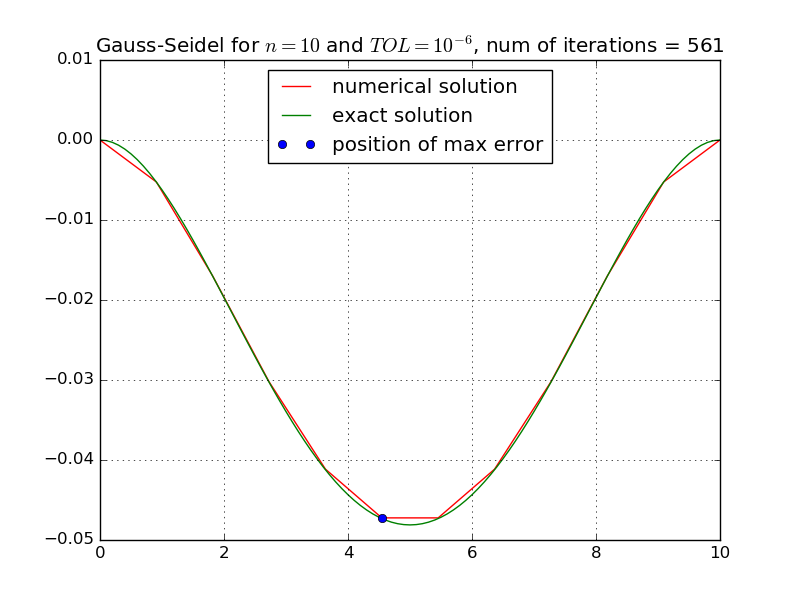
\includegraphics[width=0.8\textwidth]{n_10.png}
	 			\caption{Vergleich numerische und analytische Lösung}
	 			\label{fig:Bild1}
	 		\end{figure}
	 		Für eine 6-Stellige Genauigkeit werden 561 iterationen benötigt. Dabei beträgt der Fehler, welcher in der Mitte des Balkens liegt, ca.
	 		$8.75913330772e^{-5}$.
	 	
	 	\subsubsection{Auswertung für k's}
	 		Nun werden die Gleichungssysteme mittels $multi\_solve$ gelöst. Zunächst werden dabei die Parameter $max\_iter=10000$ und $tol=1e^{-6}$ verwendet. Die Auswertung liefert folgende Fehlertabelle für den Fehler in der Mitte des Balkens.	 		
			\begin{table}[!h]
				\centering
				\begin{tabular}{c c c c}
					\bf k & \bf Fehler\\
					\hline
					1	& 4.0104791661e-05 \\ 
					2   & 0.0285147270488 \\
					3	& 0.0467199915587 \\
					4	& 0.0480244275509\\
					5   & 0.0481081478527\\
					6	& 0.0481135140356\\
				\end{tabular}
			\end{table}
			Man kann erkennen, dass bereits für relativ kleine $k$ der Fehler recht groß wird. Bereits ab $k=3$ ist das Resultat für die genutzen Parameter unbrauchbar. Der Grund hierfür liegt darin, dass für große $n$ das Verfahren nur sehr langsam konvergiert. Der Plot für $k=1..10$ verdeutlicht die Situation.
		 	\begin{figure}[H] 
	 			\centering
	 			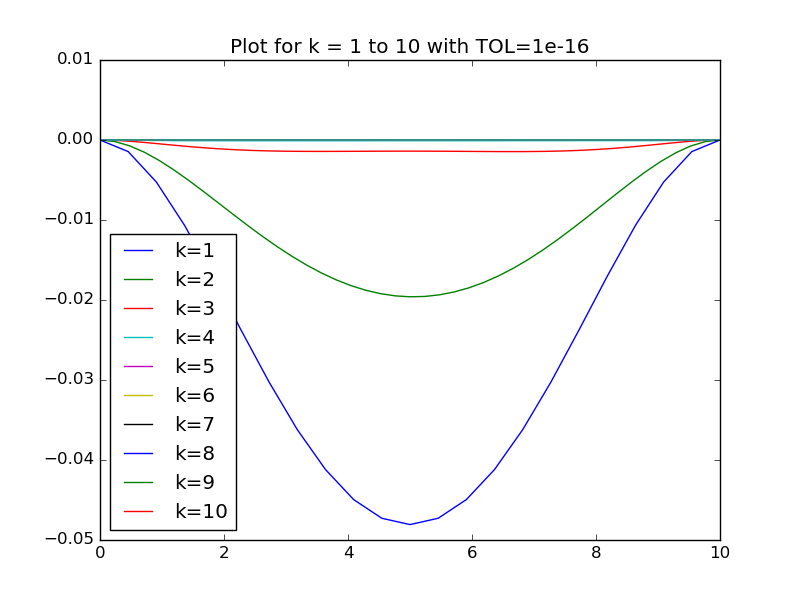
\includegraphics[width=0.9\textwidth]{ks.png}
	 			\caption{Plots für k=1..10}
	 			\label{fig:Bild2}
	 		\end{figure}
	 		Bereits ab $k=2$ kann man im Plot sehen, dass das Resultat nicht zufriedenstellend ist da der Fehler viel zu groß wird. Abhilfe verschaffen hierfür besser geeignete Parameter. Die folgende Auswertung verwendet die Parameter $max\_iter=1000000$ und $TOL = 1e^{-100}$. Die Rechenzeit betrug dabei $t \approx 8h$
			\begin{table}[H]
				\centering
				\begin{tabular}{c c c c}
					\bf k & \bf Fehler\\
					\hline
					1	& 1.27883814649e-14 \\ 
					2   & 1.7937734631e-13 \\
					3	& 0.00121666321593 \\
					4	& 0.0382262076262\\
					5   & 0.0475469272666\\
					6	& 0.0480776249649\\
				\end{tabular}
			\end{table}
			\newpage
			Es zeigt sich, dass die Näherungen besser werden. Jedoch ist bereits ab $k=4$ die Anzahl an iterationen mit $max\_iter=1000000$ zu niedrig angesetzt. Der Plot verdeutlicht, dass selbst nach so langer rechenzeit, die Ergebnisse nicht merklich besser werden.	 		
		 	\begin{figure}[H] 
	 			\centering
	 			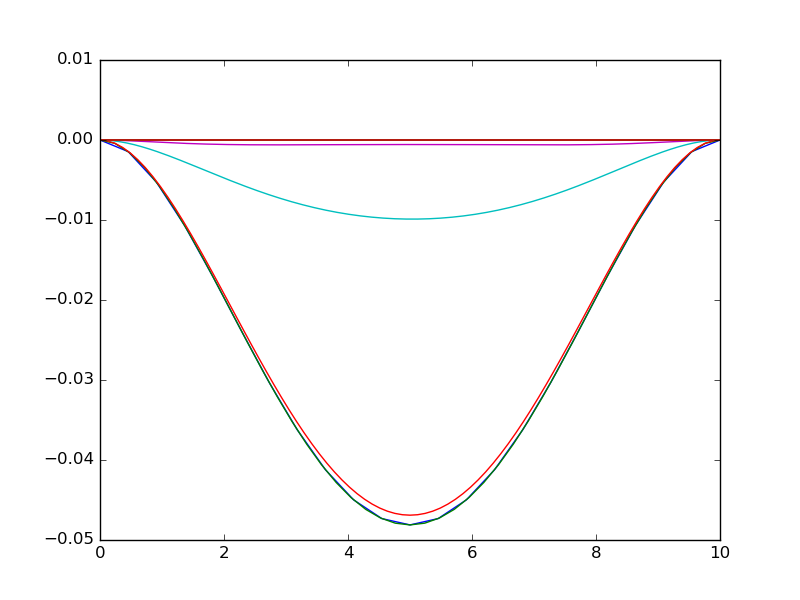
\includegraphics[width=0.9\textwidth]{one_mill.png}
	 			\caption{Plots mit max\_iter = 1000000}
	 			\label{fig:Bild3}
	 		\end{figure}
	 		
	 		Bereits für kleine k wird der Fehler in der Mitte des Balkens sehr schnell, sehr groß.
	 		
	 		\subsubsection{Fehlerbetrachtung}
				Die Kondition sagt etwas darüber aus ob kleine störungen zu verstärkung des Fehlers über alle Grenzen führen. Wenn für den Konditionswert gilt $K(A) < 1$ so spricht man von
				einem gut Konditionierten (bzw. gut gestelltem) Problem. Für reguläre Matrizen lässt sich der Konditionswert abschätzen durch
				\begin{equation}
					K(A) = \norm{\norm{A}}\cdot\norm{\norm{A^{-1}}}.
				\end{equation}
				Hierfür muss jedoch gelten, dass für beliebig große Gleichungssysteme die Matrix $A$ regulär ist (also vollen rang hat). Dies gilt genau dann wenn
				\begin{equation*}
					det(A) \neq 0.
				\end{equation*}
				\newpage
				Begründen lässt sich dies wie bereits bei der Konvergenzuntersuchung. Da alle diagonalen, bis auf die Hauptdiagonale, mindestens ein Null Element enthalten, kann
				die Determinante wie folgt dargestellt werden
				\begin{equation*}
					12\cdot\prod_{i=1}^{n-1}6 \cdot 12.
				\end{equation*}
				Dieser Ausdruck ist immer größer als $0$, somit ist $A$ für beliebige größen regulär. Also kann Gleichung (4) zur bestimmung der Kondition verwendet werden.
				
			\subsubsection{Konditionsbestimmung}
				Die Kondition des Problems für verschiedene $k$ soll mit Hilfe von Python bestimmt werden. Hierfür werden die Funktionen $norm$ und $inv$ aus dem Paket $numpy.linalg$ verwendet.
				Notwendigerweise werden nun die Matrizen tatsächlich konstruiert, dies geschieht mittels der Funktion $create\_matrix$ welches als Parameter die Dimension $n$ erwartet.\newline
				\newline
				\begin{tabular}{c}
				\begin{lstlisting}
def create_matrix(n):
   	matrix = [[] for _ in range(n)]
    matrix[0] = [12, -6, 4.0/3.0] + [0 for _ in range(n-3)]
    matrix[1] = [-4, 6, -4, 1] + [0 for _ in range(n-4)]
    matrix[n-2] = [0 for _ in range(n-4)] + [1, -4, 6, -4]
    matrix[n-1] = [0 for _ in range(n-3)] + [4.0/3.0, -6, 12]
    for j in range(2, n-2, 1):
      matrix[j] = [0 for _ in range(j-2)] + [1, -4,  6, -4, 1] + [0 for _ in range(n-3-j)]
    return matrix	
	 			\end{lstlisting}
				\end{tabular}
				\newline \newline
				Die so erzeugten Matrizen werden verwendet um mittels Gleichung (4) den Konditionswert für das jeweilige Gleichungssystem zu bestimmen.
				Große Konditionswerte bedeuten langsames Konvergenzverhalten.
				Zur berechnung der Konditionen wird die Funktion $compute\_conditions$ verwendet, welche ein oberes Limit für den Wert $k$ bekommt.
				Als Resultat wird eine Liste mit den entsprechhenden Konditionswerten zurückgeliefert. \newline \newline
				\begin{tabular}{c}
				\begin{lstlisting}
				def compute_conditions(k_limit):
    				n_list = [10 * (2**k) + 1 for k in range(1, k_limit+1, 1)]
    				cond_list = [0 for _ in n_list]
    				for n in n_list:
        				index = n_list.index(n)
       					matrix = create_matrix(n)
        				inverse_matrix = nplin.inv(matrix)
        				matrix_norm = nplin.norm(matrix)
        				inverse_matrix_norm = nplin.norm(inverse_matrix)
        				cond_list[index] = matrix_norm*inverse_matrix_norm
    				return cond_list
				\end{lstlisting}
				\end{tabular}
				\newline \newline
				Die Funktion bildet zu jeder Matrix die Inverse und bestimmt die jeweiligen Normen.
				\newpage
				Ein Plot der die Kondition zu jedem Wert für k darstellt, verdeutlicht das Verhalten.
				\begin{figure}[H] 
					 \centering
					 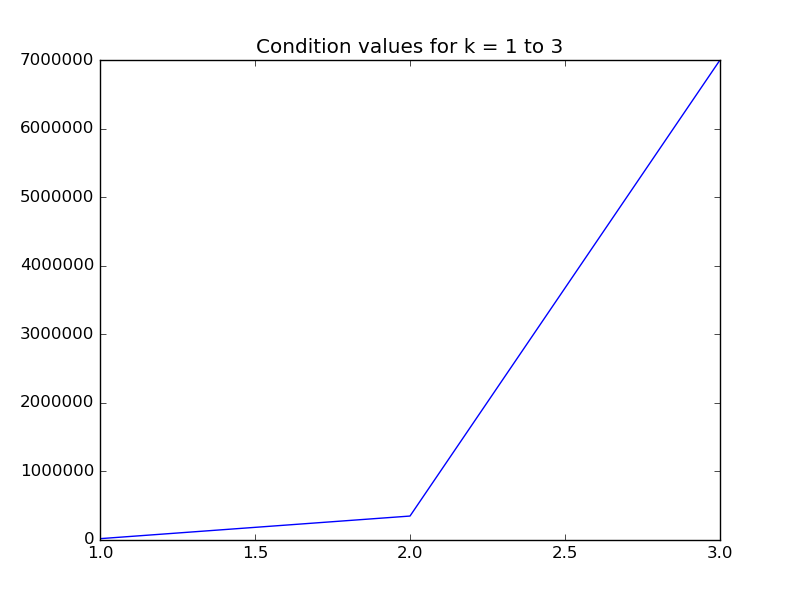
\includegraphics[width=0.9\textwidth]{conds.png}
					 \caption{Plots mit Konditionen}
					 \label{fig:Bild4}
				\end{figure}
				
\section{Belasteter Balken}

	Nun soll der aufliegende Balken zwischen $x=3$ und $x=4$ zusätzlich mit 500$kg$ belastet werden.
	Da die angreifende Kraft bereits als eine Liste in den Algorithmen implementiert wurde ist es aussreichend die rechte Seite vor
	dem Ausführen der Routinen anzupassen. Hierfür wird die Funcktion $apply\_weight\_to\_f$ verwendet. Diese erhält als Argumente die Liste mit
	den standartmäßig wirkenden Kräften $fs$, als auch eine Schrittweite $h$. Für jedes Element dessen tatsächliche Position zwischen $x=3$ und $x=4$ liegt
	wird die zusätzliche Belastung von 500$kg$ addiert. \newline \newline
	\begin{tabular}{c}
	\begin{lstlisting}
		def apply_weight_to_f(fs, h):
    		for i in range(len(fs)):
        		if 3 <= h*i <= 4:
            		fs[i] += 500
	\end{lstlisting}
	\end{tabular}
	\newline \newline
	Die Funktion hat keinen Rückgabewert da sie den Zustand der Liste selbst verändert.	
	
	\subsection{Auswertung}
		Da nun keine exakte Lösung vorhanden ist an der ein Fehler gemessen werden kann, wird in diesem Teil darauf verzichtet.
		Stattdessen wird die Verschiebung der maximalen Auslenkung untersucht. Hierfür wird die Routine $multi\_solve$ mit angepasster rechter Seite
		ausgeführt. Diesmal werden jedoch die Parameter $max_iter=100000$ und $tol=1e^{-18}$ verwendet.
		
		\subsubsection{Auswertung n = 10}
			Der Vergleich beider numerischen lösungen, mit extra gewicht und ohne, liefert folgenden Plot.
			
		\begin{figure}[H] 
	 		\centering
	 		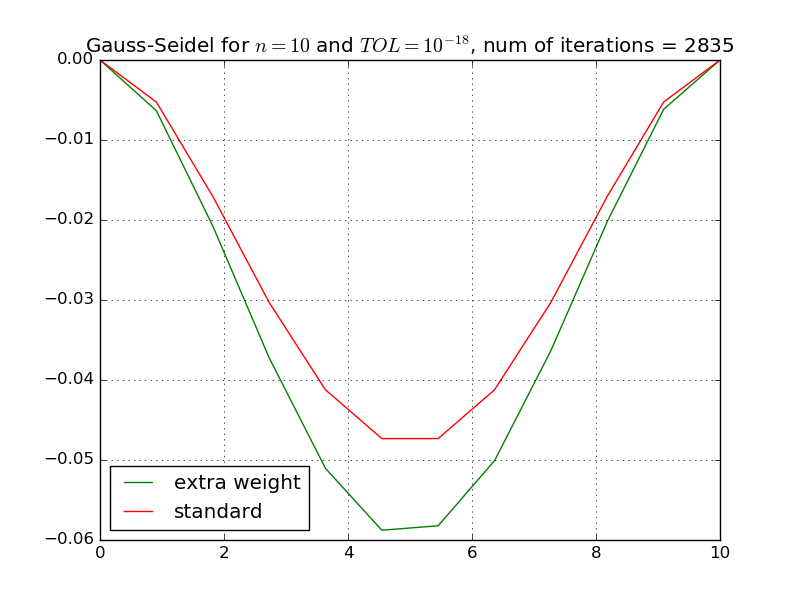
\includegraphics[width=0.9\textwidth]{bend.png}
	 		\caption{Plots mit max\_iter = 1000000}
	 		\label{fig:Bild5}
	 	\end{figure}
	 	
	 	Es ist erkenntlich, dass der Punkt mit der größten Auslenkung für $n = 10$ sich nicht verändert hatt, jedoch der Betrag der Auslenkung gewachsen ist.
	 	Deutlicher wird die Linksverschiebung der größten Auslenkung für größere $n$.
	 	\newpage
	 	\subsubsection{Auswertung für k's}
	 		Dieses mal werden nur $k<=5$ ausgewertet um die Berechnungen in einem zeitlichen Rahmen halten zu können. Für die Konvergenzgeschwindigkeit spielt die rechte Seite, 
	 		in diesem Fall, eine untergeordnete Rolle. Somit ist nicht zu erwarten dass die Resultate diesmal besser, oder schneller sind. Die Berechnungen werden mit einer
	 		angepassten $multi\_solve$ Funktion durchgeführt (nur anpassung bezüglich der Ausgabe, keine algorithmischen).
		\begin{figure}[H] 
	 		\centering
	 		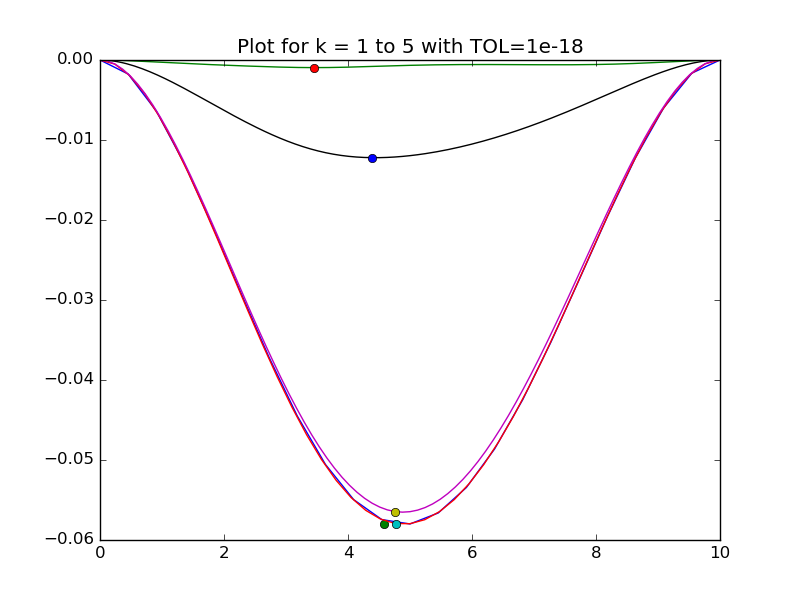
\includegraphics[width=0.9\textwidth]{extra_k.png}
	 		\caption{Plots mit max\_iter = 1000000}
	 		\label{fig:Bild6}
	 	\end{figure}
	 	Dem Plot kann entnommen werden, dass sich der Punkt mit maximaler Auslenkung tatsächlich leicht nach Links verschiebt. Nähmlich zwischen $x=4$ und $x=5$

\newpage
\section{Erklärung}
	Alexander Knoll: Mein Anteil an der Abgabe bestand in der Bearbeitung der Aufgaben Eins bis Fünf. Dazu gehört die umsetzung in Python als auch die Dokumentation in TeX.

%\newpage
%\bibliography{literatur}
%\bibliographystyle{agsm}

%\begin{thebibliography}{xxxxxxxxxxxxxxxxxxxxxxxxxxxxxxxxxxxxxx}


%\end{thebibliography}

\end{document}